\documentclass[12pt,twoside]{article}
\usepackage{jmlda}
\usepackage{hyperref}       % clickable links
\usepackage{Iv_commands}    % you can delete this
\usepackage{tikz}
\usepackage{verbatim}
\usepackage{rotating}
\usepackage{hyperref}
\usepackage{xcolor}
\hypersetup{%
  colorlinks=true,% hyperlinks will be coloured
  linkcolor=red,% hyperlink text will be green
  linkbordercolor=red,% hyperlink border will be red
}

\usetikzlibrary{calc,trees,positioning,arrows,chains,shapes.geometric,%
    decorations.pathreplacing,decorations.pathmorphing,shapes,%
    matrix,shapes.symbols}

\tikzset{
>=stealth',
  punktchain/.style={
    rectangle, 
    rounded corners, 
    % fill=black!10,
    draw=black, very thick,
    text width=10em, 
    minimum height=3em, 
    text centered, 
    on chain},
  line/.style={draw, thick, <-},
  element/.style={
    tape,
    top color=white,
    bottom color=blue!50!black!60!,
    minimum width=8em,
    draw=blue!40!black!90, very thick,
    text width=10em, 
    minimum height=3.5em, 
    text centered, 
    on chain},
  every join/.style={->, thick,shorten >=1pt},
  decoration={brace},
  tuborg/.style={decorate},
  tubnode/.style={midway, right=2pt},
}

\newcommand{\hdir}{.}
\renewcommand{\L}{\mathcal{L}}
\newcommand{\lto}{\leftarrow}



\theoremstyle{plain}
\newtheorem{thm}{Теорема}[section]
\newtheorem{lem}{Лемма}[section]

\theoremstyle{remark}
\newtheorem{rem}{Ремарка}[section]

\theoremstyle{definition}
\newtheorem{df}{Определение}[section]

% version 0.5

\title
    {Синергия алгоритмов классификации (SVM Multimodelling)}
\author
    {С.\,~Иванычев, А.\,~Адуенко}
\email
    {\href{mailto:sergeyivanychev@gmail.com}{sergeyivanychev@gmail.com},  \href{mailto:aduenko1@gmail.com}{aduenko1@gmail.com}}
\organization
    {Московский физико-технический институт}
\abstract
    {В данной статье рассматривается проблема агрегирования небольшого количества сильных классификаторов с целью улучшения решений задач классификации и регрессии.  В качестве примера подобной системы рассматривается система SVM  алгоритмов использующая kernel-trick с различными ядрами. Для комбинации решений и улучшения качества прогнозирования в задачах классификации и регрессии (SVR) авторы предлагают способ формирования новых признаков на основе сгенерированных отступов (\emph{margins}) каждым классификатором, приводят алгоритм обучения на полученных объектах и анализируют отличия множеств опорных объектов для различных ядер. В качестве практической проверки были проведены эксперименты на различных реальных данных из репозитория UCI.

    \bigskip
\noindent
\textbf{Ключевые слова}: \emph {двухклассовая классификация, композиция алгоритмов, SVM, SVR, бэггинг}
}

\bibliographystyle{unsrt}

\begin{document}
\maketitle

\section{Введение}
Работа посвящена комбинированию небольшого количества сильных SVM, использующих kernel-trick с различными ядрами и получению агрегированного классификатора для улучшения решений задач классификации и регрессии.

    SVM(Support Vector Machine) или \emph{метод опорных векторов}\cite{Cortes1995, Boser1992} ---~это один из наиболее распространенных и эффективных методов в машинном обучении, которые используется для задач классификации и регрессии (SVR). Задача математического программирования сводится к двойственной задаче, функционалы в которой не зависят от векторов признаков как таковых, а лишь от их попарных скалярных произведений. Использование особых функций, \emph{ядер}, то есть скалярных произведений в сопряженном пространстве, позволяет получить разделяющие поверхности между классами более сложной формы \cite{Smola2004}. Наша цель --- скомбинировать SVM
    с различными примененными ядрами для улучшения решения, а также анализ множеств опорных объектов в случае разных использованных ядер.

    Наиболее классическими методами агрегирования алгоритмов являются
    бэггинг (\emph{bagging})\cite{Breiman1996} и бустинг (\emph{boosting}) \cite{Freund1995}, и их
    вариации, однако они работают только с  большим количеством слабых классификаторов, что делает невозможным использование его использование для указанного множества базовых алгоритмов.

    Среди способов агрегации для небольшого количества классификаторов можно
    выделить, например, выбор большинства классификаторов \cite{Franke1992},
    комбинирование ранжирований (rankings) по классам, сделанных различными
    классификаторами \cite{Ho1994}. В дальнейшем было показано, что все подобные
    методы есть особые случаи составного классификатора из \cite{Kittler1996},
    появляющиеся при особых условиях или способах аппроксимации.

    Различные способы агрегации SVМ используются во многих задачах анализа данных.
    \cite{Martin-merino2007} использовали совокупность SVМ для уменьшения ошибочно негативных классификаций (FP) в задаче фильтрации спама среди электронных писем.
    Для этого на электронных письмах были введены различные метрики, для каждой из них был приспособлен SVM, а затем результат получался голосованием \cite{Kittler1996}.
    \cite{Gorgevik2005}, решавшие задачу распознавания написанных рукой символов, делили множество признаков на четыре непересекающихся подмножества, и на каждом из них обучали SVM, увеличив этим самым коэффициент распознавания по сравнению с одним SVM.

    В последнее время стал набирать популярность \emph{метод многоядерного обучения} (MKL,~multiple kernel learning) \cite{Dyrba2015, Bucak2014,Althloothi2014}, который основывается на том, что линейная комбинация ядер также является ядром. Данный метод хорош при объединении данных из нескольких источников и полной автоматизации, так как суперпозиция функций может быть оптимизирована любым методом валидации (например кросс-валидацией).

    Мы также предлагаем использовать накопившийся банк ядер, однако не на этапе обучения SVM, а на этапе агрегирования обученных алгоритмов. Известно, что алгоритм $b_i$ для объекта $x_j$ обучающей выборки генерирует \emph{отступ} (margin). По отступу в общем случае можно определить не только предсказанный класс, но и насколько <<уверен>> в своем решении алгоритм. В случае банка с $n$ ядрами и обучающей выборки с $m$ сэмплами
    мы получим матрицу отступов $M \in \R^{m\times n}$. Отнормировав ее, мы получим новую матрицу <<объект-признак>>, где вектором признаков каждого объекта будет вектор отнормированных отступов.

    В этой работе предложен алгоритм обучения на матрице отступов, проведен анализ опорных объектов, генерируемые различными ядрами, а также проведено тестирование полученного алгоритма на реальных данных репозитория UCI.


\section{Постановка задачи}

Пусть $X^l = \brs{\vec{x}_i, y_i}_{i=1}^l$~---~обучающая выборка, $\vec{x}\in \R^n, y \in \{\pm 1\}$.

\begin{df}
	Под $s$-й \emph{моделью} будем понимать SVM с
ядром $K_s$ где выбрано множество ядер:
$$
\mathcal{K} = \{K_i\}_{j=1}^m
$$
\end{df}
	
При обучении каждая модель дает классификатор или регрессор (в зависимости от типа $Y$). Например, для случая $Y \in \{-1, +1\}$ классификации алгоритм выглядит следующим образом:

\begin{equation} \label{decision}
	b_s(\v{x}) = \sign\sbrs{\sum_{i=1}^l\lambda_i y_i K_s(\vec{x}_i, \vec{x}) - w_0}
\end{equation}

Где $\{\lambda_i\}$ и $w_0$ находятся из решения задачи математического программирования\cite{Smola2004}

\begin{equation*}
 \begin{cases}
   \sum_{i=1}^l \lambda_i + \frac{1}{2}\sum_{i=1}^{l}\sum_{j=1}^{l}
    \lambda_i \lambda_j y_i y_j K_s(\vec{x}_i, \vec{x}_j) \to \min_\lambda
   \\
   0 \leq \lambda_s \leq c, \;\; i = 1\ldots l
   \\
   \sum_{i=1}^l\lambda_i y_i = 0
 \end{cases}
\end{equation*}

Результатом обучения является то, что модель для обучающей выборки генерирует вектор \emph{отступов} (margins) для каждого объекта. 
$$
M_s = \sum_{i=1}^l\lambda_i y_i K_s(\vec{x}_i, \vec{x}) - w_0
$$
Совокупность отступов порождает матрицу отступов  размерности
$M \in \R^{l\times m}$,
в котором $(i, j)$-й элемент ---~это отступ $i$-го объекта в SVM с~$j$-м ядром. Авторы утверждают, что эта матрица может быть использована как новая обучающая выборка для построения агрегирующего алгоритма.

Рассмотрим $M$ как новую матрицу <<объект-признак>>, $\mathcal{A}$ ---~ множество алгоритмов
вида
\begin{equation}
    \mathcal{A} = \fbrs{a(\vec{x}) = g(\vec{x}, \theta)|\theta \in \Theta}\;\; g:\R^m \to Y
\end{equation}
где $\Theta$ --- некое семейство параметров.
\begin{df}
Пару $(g, \mathcal{K})$ назовем \emph{мультимоделью}.
\end{df}

$L(y, y^*)$ ---~функционал качества. Тогда перед нами стоит 
Задача выбора алгоритма агрегирования сильных классификаторов супермодели:
	\begin{equation}
    	L(y, g(M(X), \theta)) \to \min_{\Theta}
	\end{equation}

В качестве этой функции мы предлагаем использовать площадь под ROC-кривой (AUC-ROC) как устойчивый к несбалансированностям в выборке.
\section{Близость моделей}

Так как агрегация сильных классификаторов должна быть устойчива к похожим моделям в ее составе, она должна каким-то образом определять идентичные SVM. В данной секции попробуем установить связь между корреляцией векторов отступов,
генерируемых
разными ядрами на одной и той же обучающей выборке и степенью <<похожести>>
ядер. Понятие <<похожести>> или близости отождествляется с введением метрики
на пространстве ядер. 
\begin{df}
	\emph{Расстоянием между ядрами} $\rho(K_i, K_j)$ на выборке $X^l$ будем называть функцию:
$$
\rho_{X^l}(K_i, K_j) = \frac{\#\sbrs{\mathrm{SV}_i \;\Delta\; \mathrm{SV}_j}}
{\#\sbrs{\mathrm{SV}_i \cup \mathrm{SV}_j}}
$$
Где под $\mathrm{SV}_j$ понимается множество опорных объектов на $j$-м ядре, под
знаком $\Delta$ --- симметрическая разность.
\end{df}
\begin{df}
	\emph{Похожестью SVM с ядрами} $K_i, K_j$ будем называть следующую функцию
$$
s_{X^l}(K_i, K_j) = 1 - \mathrm{corr}(M_i, M_j)
$$	
где под $M_i$ понимается вектор отступов соответственного SVM, а функция $\mathrm{corr}(\cdot, \cdot)$ --- корреляция Пирсона. 
\end{df}

В качестве исходных данных
возьмем датасеты Wine \cite{UCI:Wine}, German credit data\cite{UCI:German} и
Heart disease\cite{UCI:Heart}. Варьируя коэффициент L2-регуляризации, в качестве базового набора ядер возьмем

\begin{itemize}
    \item Линейное
    \item Полиномиальное (степени 3, 4, 5)
    \item RBF-ядро ($\gamma \in \{0.0001, 0.001, 0.01, 0.1, 1\}$)
\end{itemize}

Для каждого значения коэффициента регуляризации построим графики
опишем полученное множество классификаторов.

% Выглядит очень разумно. Напиши какие-то выводы.
% Опиши, для какого датасета 
% - сколько векторов, 
% - насколько в среднем похожи, 
% - насколько результаты для разных ядер похожи, 
% - насколько похожи их множества опорных объектов.

% Опиши, как влияет параметр С, сделай глобальный вывод применительно ко всем датасетам, какие пары ядер дают схожие результаты.
% Укажи на различия, где различия в векторах напрямую дают различие в ответах, а где нет и в попробуй определить, почему.

\newpage

\subsection{German credit dataset}

\begin{figure}[H]
      \center{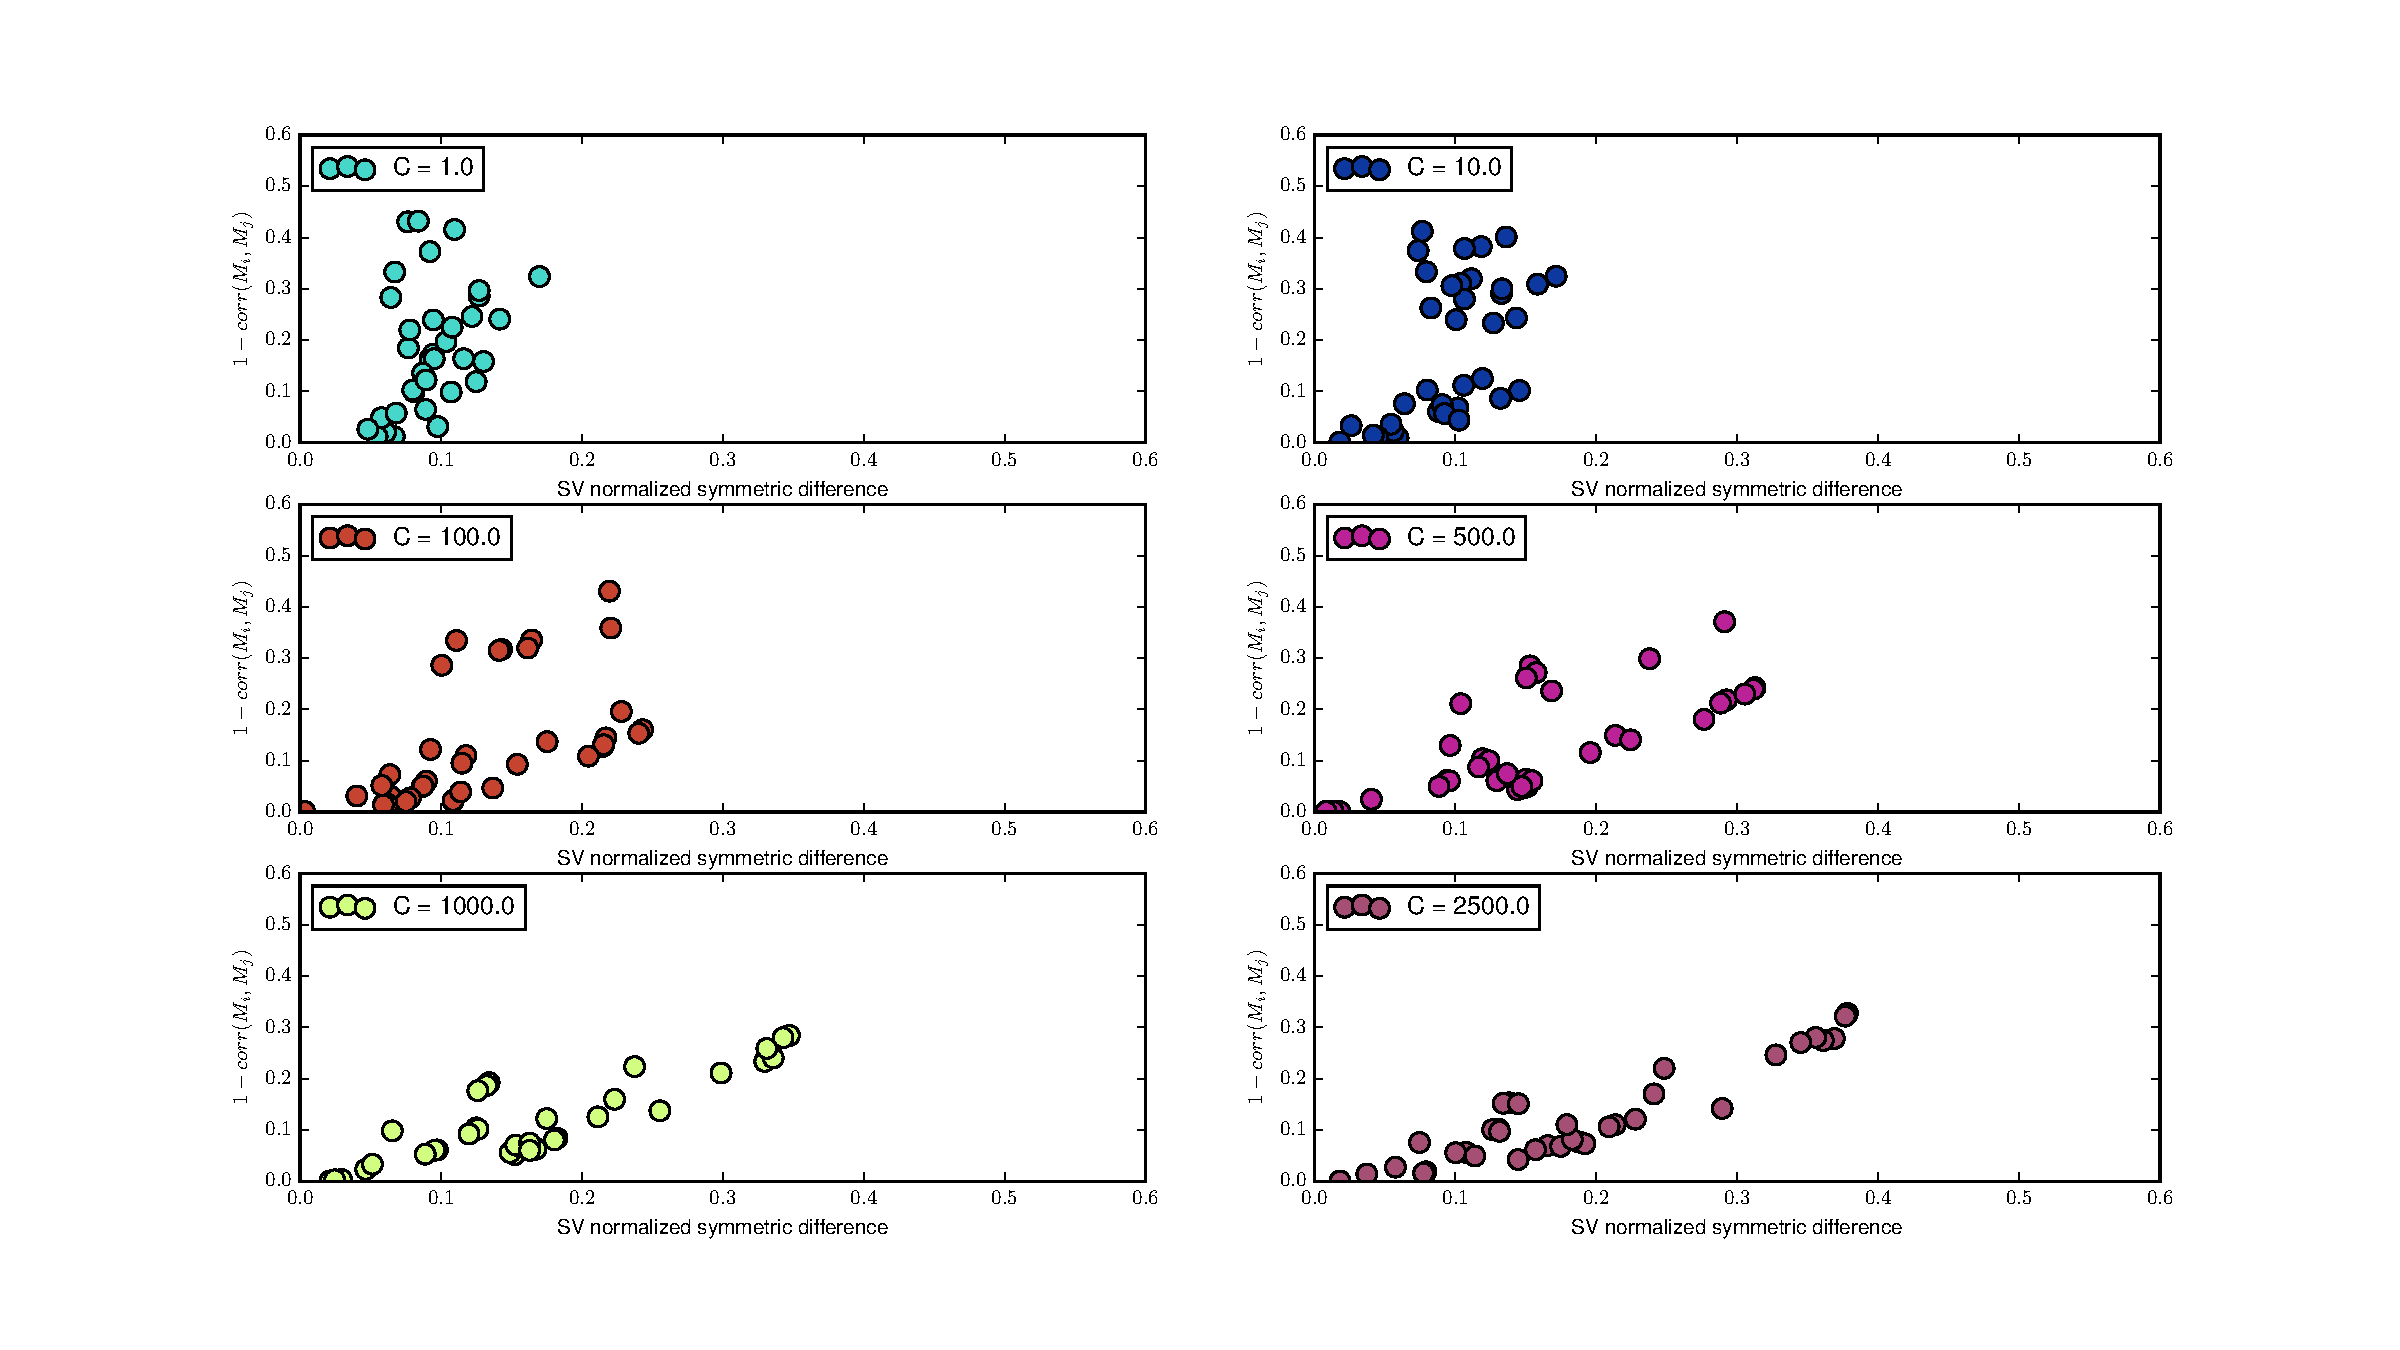
\includegraphics[width=\textwidth]{german.pdf}}
      \caption{German credit}
\end{figure}

\input{german.tex_table}


Обучающая выборка состоит из 1000 семплов по 24 числовых признака. 

\newpage

\subsection{Wine dataset}


\begin{figure}[H]
      \center{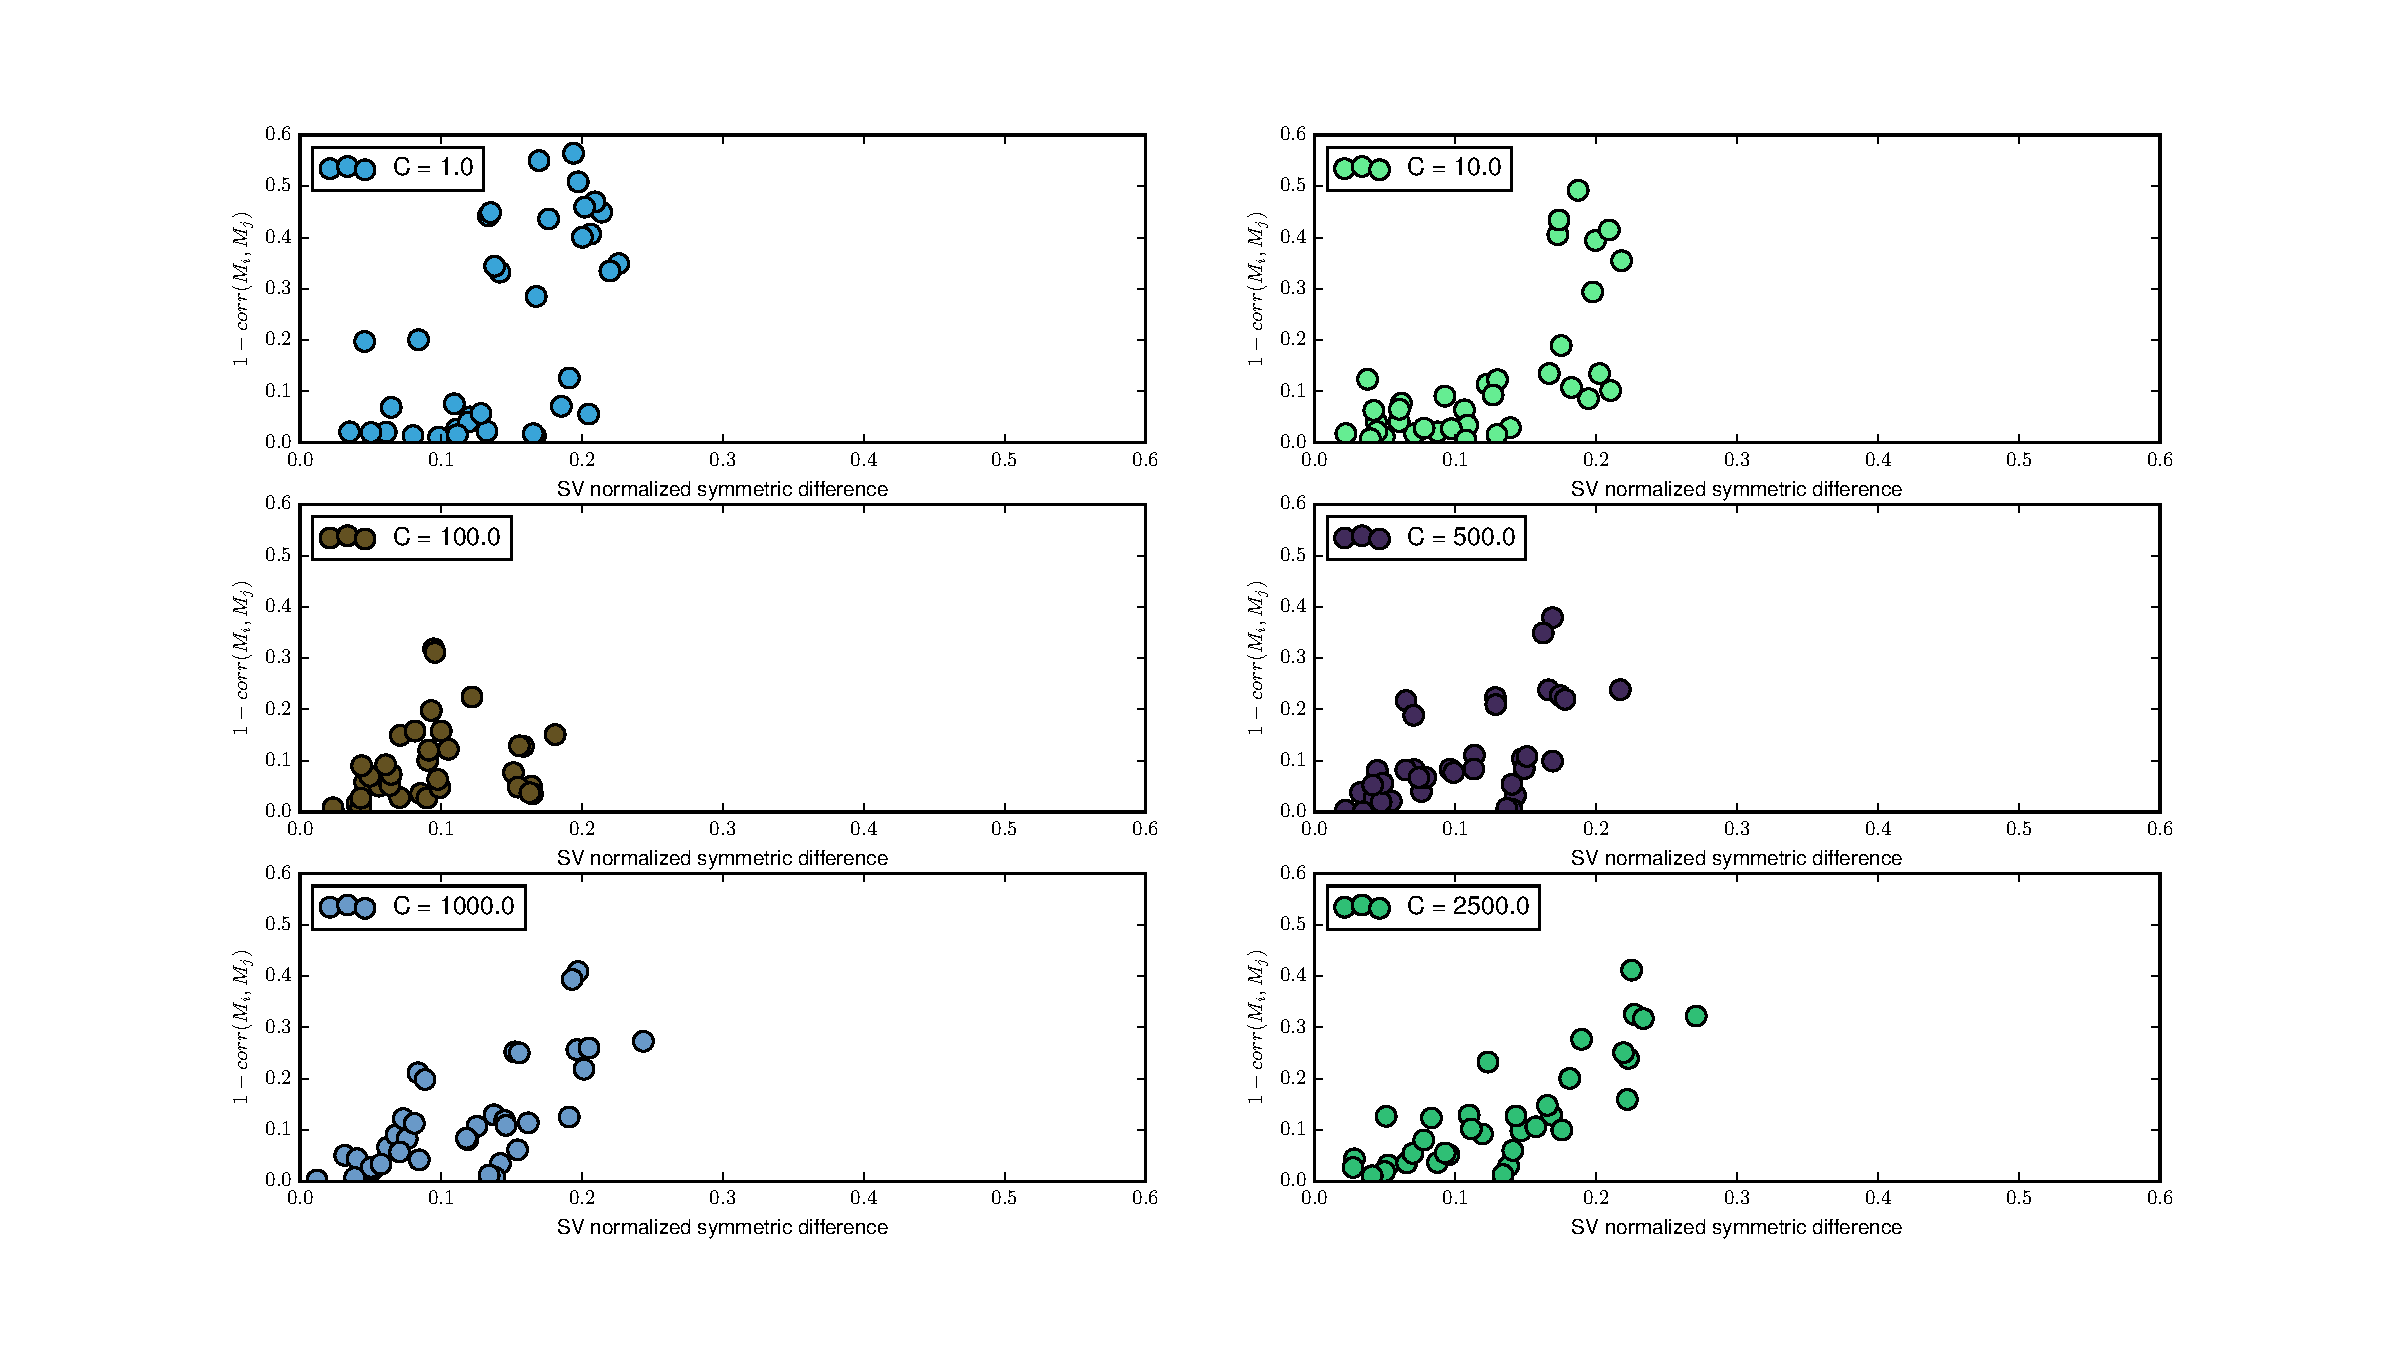
\includegraphics[width=\textwidth]{wine.pdf}}
      \caption{Wine quality}
\end{figure}

\input{wine.tex_table}


\newpage

\subsection{Heart dataset}

\begin{figure}[H]
      \center{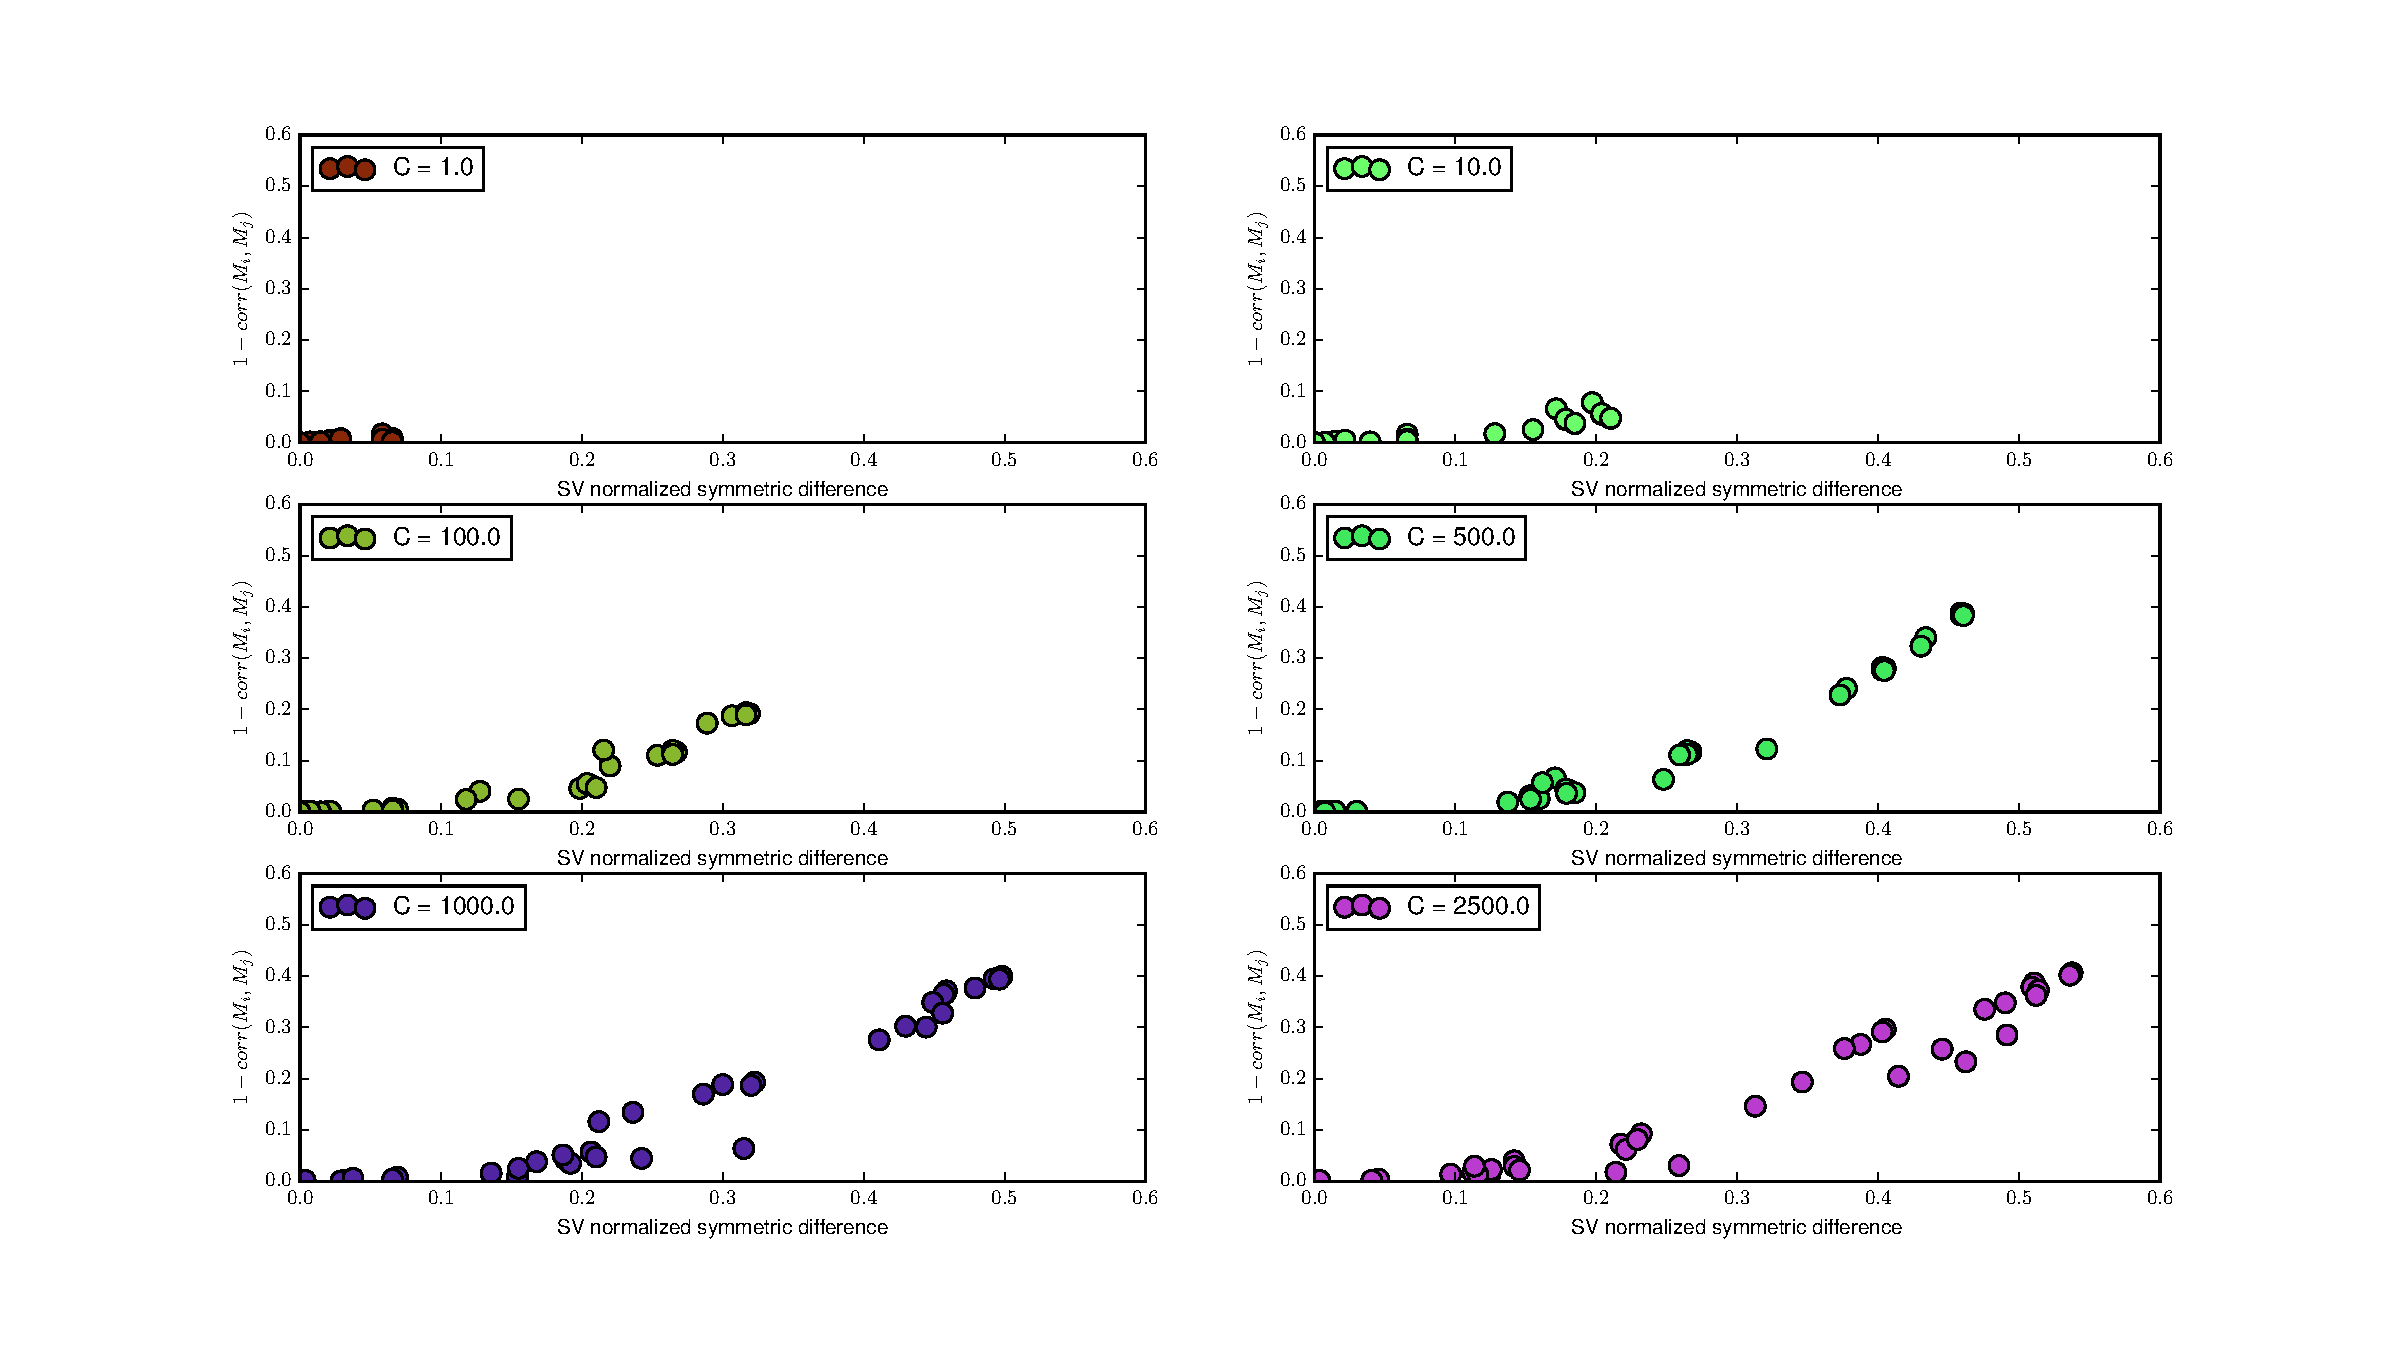
\includegraphics[width=\textwidth]{heart.pdf}}
      \caption{Heart disease}
\end{figure}

\input{heart.tex_table}

\subsection{Выводы из эксперимента}

Уже по этим данным можно сказать, что

\begin{itemize}
  \item С ростом константы регуляризации расстояние между ядрами и расстояние между	
  их отступами лучше коррелируют между собой.
  \item При высоких параметре регуляризации коэффициент корреляции Пирсона 
  достигает более $0.8$, то есть расстояния практически линейно зависят друг от друга.
  \item Вектора средних ядерных и отступных расстояний кореллируют по-разному на различных датасетах (на Wine и Heart корелляции Пирсона $0.85$ и $0.99$ соответственно, на German --- $-0.92$).
\end{itemize} 

\newpage

\subsection{Решение задачи. Модели}

В качестве множества ядер $\mathcal{K}$, участвующих в мультимодели выберем следующий набор.

\begin{itemize}
    \item Линейное
    $$
    K_{\text{linear}}(\v{x}, \v{x'}) = \rbrs{\v{x}, \v{x'}}
    $$
    \item Полиномиальное (степени 3, 4, 5)
    $$
    K_{d\text{-poly}}(\v{x}, \v{x'}) = (\rbrs{\v{x}, \v{x'}} + 1)^d
    $$
    \item RBF-ядро (\emph{Radial basis function}) ($\gamma \in \{0.0001, 0.001, 0.01, 0.1, 1\}$)
    $$
    K_{\text{RBF}}(\v{x}, \v{x'}) = e^{-\gamma ||\v{x} - \v{x'}||^2}
    $$
    \item INK-spline ядро\cite{Izmailov2013} (степени 1, 2)
    $$
K(x, y) = \sum_{r=0}^{d} (x-a)^r(y-a)^r + \sum_{r=0}^{d} \frac{1}{2d - r + 1} \begin{pmatrix} d\\r \end{pmatrix}
(|x - y|)^r(\mathrm{min}(x, y)  - a)^{2d - r + 1}
$$

$$
\mathbf{K}(\mathbf{x}, \mathbf{x'}) = \prod_{j=1}^n K_j(x_j, x'_j)
$$

$$
K_{\text{INK}}(\mathbf{x}, \mathbf{x'}) = \frac{\mathbf{K}(\mathbf{x}, \mathbf{x'})}{\sqrt{\mathbf{K}(\mathbf{x}, \mathbf{x})
\mathbf{K}(\mathbf{x'}, \mathbf{x'})}}
$$
\end{itemize}

Данное множество выбрано как наиболее универсальные представители различных классов ядер. 

\subsection{Виды мультимоделей. Логистическая регрессия (logregr).}

Базовым вариантом агрегирующего алгоритма является логистическая регрессия обученная на всей обучающей выборке $X^l$. Эта модель характеризуется оптимизационной задачей

\begin{equation}\label{logregr}
	R(w) + C \sum_{i=1}^n \log(\exp(- y_i (X_i^T w + c)) + 1) \to \min_{w, c}
\end{equation}

где $R(w)$ --- регуляризатор.
Здесь для большей наглядности будем пользоваться обозначениями $X_{\text{train}}, y_{\text{train}}, X_{\text{test}}$. Опишем процессы обучения супермодели и предсказания.

\vspace{0.5cm}

\begin{figure}[!ht]
  \centering
      \begin{tikzpicture}
  [node distance=.8cm,
  start chain=going right,]
     \node[punktchain, join] (svm) {Обучение моделей на $X_{\text{train}}$};
     \node[punktchain, join] (margin)      {Подсчет отступов для объектов из $X_{\text{train}}$. Генерация матрицы $M_\text{test}$};
     \node[punktchain, join] (super)      {Обучение логистической регрессии на $M_\text{train}$};
  \end{tikzpicture}
  \caption{Обучение (logregr)}
\end{figure}

\begin{figure}[!ht]
  \centering
      \begin{tikzpicture}
  		[node distance=.8cm,
  		start chain=going right,]
     \node[punktchain, join] (margin)      {Подсчет отступов для объектов из $X_{\text{test}}$. Генерация матрицы $M_\text{test}$};
     \node[punktchain, join] (super)      {Предсказание супермоделью по матрице $M_\text{test}$};
  \end{tikzpicture}
  \caption{Предсказание (logregr)}
\end{figure}

Данный подход зарекомендовал себя как склонный к переобучению, так как при наличии практически идеального классификатора в супермодели, например, переобученного на $X_\text{train}$, логистическая регрессия будет давать ему на обучении большие веса, тем самым также переобучаясь.

\section{Stacked generalization (logregr + stacking)}

Для того, чтобы избежать переобучения мы применим \emph{стэкинг}\cite{Wolpert} (stacking). Обучающую выборку разделим на две подвыборки $X_\text{train}$ и $X_\text{validate}$. На первой из них обучаем SVM, а на предсказанных отступах другой половины обучаем логистическую регрессию.

\begin{figure}[!ht]
  \centering
      \begin{tikzpicture}
  [node distance=.5cm,
  start chain=going right,]
  	\node[punktchain, join] (svm) {Деление $X^l$ на $(X_\text{train}, y_\text{train})$ и $(X_\text{val}, y_\text{val})$};
     \node[punktchain, join] (svm) {Обучение моделей на $X_{\text{train}}$};
     \node[punktchain, join] (margin)      {Подсчет отступов для объектов из $X_{\text{valid}}$. Генерация матрицы $M_\text{valid}$};
     \node[punktchain, join] (super)      {Обучение логистической регрессии на $M_\text{valid}$};
  \end{tikzpicture}
  \caption{Обучение (logregr + stacking)}
\end{figure}

Процесс предсказания остался аналогичным базовому варианту. 

\section{Положительная логистическая регрессия (positive)}

Обладая множеством моделей, алгоритм, аггрегирующий их, учитывает в большей или меньшей степени каждый из классификаторов. Напомним, что логистическая регрессия сопоставляет на этапе решения оптимизационной задачи \ref{logregr} каждому признаку некоторый вес. В случае нашей задачи признаки --- это отступы классификаторов, что делает некорректным отрицательность весов. Эту проблему можно решить несколькими способами:
\begin{itemize}
	\item \textbf{(regularizer + positive)} Используем $l_1$-регуляризацию в \ref{logregr}, тем самым отбирая классификаторы, а затем откидываем те, вес которых отрицателен. То есть логистическая регрессия будет учитывать только отступы, соответствующие положительным весам $w_i$.
	\item \textbf{(robust)} Переопределим задачу минимизации \ref{logregr}, задав условие положительности весов 
	$$
	w \geq 0
	$$
	Данный вариант логистической регрессии называется \emph{робастной регрессией}.
\end{itemize}

\section{Модификации алгоритма}

Существуют различными модификации алгоритма (logregr + stacking) с нестрогими обоснованиями того, почему соответствующие изменения могут в том или ином виде улучшить работу супермодели. 

\begin{itemize}
	\item \textbf{( $\ldots$ + refit):} SVM обучаются не на всей выборке, а лишь только на ее части. После обучения логистической регрессии, обучим SVM заново уже не на $(X, y)_\text{train}$ а на всех тестовых данных $(X, y)$.
	\item \textbf{( $\ldots$ + window):} Обобщающую способность моделей в общем случае некорректно сравнивать исходя из полученных AUC для заданной обучающей выборки и тестовых данных, так как небольшое ($\approx 0.05$) отклонение функционала качества может быть статистически не значимым. Тем не менее, вероятно, существует порог для разности AUC двух моделей, после которого мы можем охарактеризовать одну модель как явно худшую другой. Предлагается задать <<окно>> $\delta$ и отсекать на этапе обучения SVM, для которых не выполняется условие
	$$
	\max\{\mathrm{AUC}_j\}_{j=1}^m - \mathrm{AUC} < \delta
	$$
	После сокращения, множество моделей обучается заново.
\end{itemize}

\section{Сравнение супермоделей}

Для сравнения супермоделей будем использовать четыре датасета: housing \cite{UCI:Housing}, german \cite{UCI:German}, heart \cite{UCI:Heart} и синтетический.  Последний создан как пример <<плохого>> датасета, на котором каждый классификатор едва лучше константного. Способ генерации синтетического датасета и порядок предобработки данных приведен в приложении. Представим результаты тестирования датасетов в общей таблице, в ячейках которой содержится разность AUC супермодели и лучшего классификатора из множества моделей:

\newpage

\begin{sidewaystable*}[!ht]
\centering
\caption{Результаты мультимоделирования}
\scriptsize
\begin{tabular}{|l|l|l|l|l|l|l|l|l|l|l|l|l|l|l|}
\hline
          & $l_2$  & $l_1$  & $l_1$|re & $l_1$| $w0.05$ & $l_1$|re|$w0.05$ & $l_1$|pos| & $l_1$|pos|re & $l_1$|pos|$w0.05$ & $l_1$|pos|re|$w0.05$ & $l_2$|rob & $l_1$|rob & $l_1$| rob|$w0.05$ & $l_1$|rob|re & $l_1$|rob|$w0.05$|ref \\ \hline
housing   & 0.003  & 0.003  & -0.001   & 0.003          & 0.002            & 0.003      & 0.001        & 0.002             & 0.002                & 0.003     & 0.003     & 0.002              & 0.002        & 0.001                 \\ \hline
heart     & -0.008 & -0.008 & -0.005   & -0.002         & -0.007           & -0.003     & -0.001       & -0.003            & -0.009               & -0.005    & -0.005    & -0.005             & -0.002       & -0.007                \\ \hline
german    & -0.002 & -0.003 & -0.004   & 0.002          & -0.030           & 0.001      & 0.002        & 0.002             & -0.027               & 0.001     & 0         & 0.001              & 0.002        & -0.023                \\ \hline
synthetic & -0.011 & -0.008 & -0.015   & -0.070         & -0.011           & -0.019     & -0.026       & -0.017            & -0.013               & -0.016    & -0.020    & -0.01              & -0.019       & -0.034                \\ \hline
\end{tabular}
\end{sidewaystable*}


\newpage

\section{Вывод}

В статье приведены новые способы агрегирования небольшого количества сильных классификаторов, а также несколько эвристик, которые должны улучшить результирующую обобщающую способность алгоритма. На данный момент полученный результат не состоятелен и не позволяет говорить о том, что мы смогли успешно скомбинировать сильные классификаторы. Метод нуждается в доработке. При успешном завершении работы необходимо обобщить алгоритм на случай $|Y| < \infty$ (многоклассовая классификация) и $|Y| = \infty$ (регрессия).

\section{Приложение}

\subsection{Исходный код}

Исходный код проекта написан на Python 3.5 с использованием библиотек scikit-learn \cite{scikit-learn}, numpy, pandas, matplotlib, scipy и стандартной библиотеки языка. Вы можете ознакомится с материалами, перейдя по \href{https://sourceforge.net/p/mlalgorithms/code/HEAD/tree/Group374/Ivanychev2016SVM_Multimodelling/}{ссылке}. Документация проекта содержится в файле \texttt{readme.md}, в соответствующих файлах папок \texttt{./code} и \texttt{./doc} а также в виде документирующих строк в модулях и объектах внутри Python-кода.

\subsection{Предобработка данных}

Все данные с репозитория UCI предобрабатывались следующим образом:

\begin{itemize}
	\item Обучающая выборка нормализуется. Стандартное отклонение и ожидаемое среднее сохраняются для преобразований тестовой выборки.
$$
		\mathrm{Mean} \lto \mathrm{mean}(\v{X}))\;\; \mathrm{Std} \lto \mathrm{std}(\v{X})
$$
$$
		\v{X} \lto \frac{\v{X} - \mathrm{Mean}}{\mathrm{Std}}
$$
	\item Отступы каждого классификатора преобразуются таким образом, чтобы средний модуль был равен 1.
			$$
			\mathrm{MeanMargins} \lto \frac{\mathrm{Margins}}{\mathrm{mean}(\mathrm{abs}(\mathrm{Margins}))}
			$$
			$$
			\mathrm{Margins} \lto \frac{\mathrm{Margins}}{\mathrm{MeanMargins}}
			$$
\end{itemize} 

\subsection{Подготовка синтетических данных}

Средние значения $AUC$ для данных из репозитория относительно велик ($\geq 0.8$), что говорит о том, что каждый классификатор прекрасно справляется с задачей классификации. Предполагается, что этих условиях улучшить результат проблематично, поэтому мы должны испытать супермодель на худших данных. Будем генерировать датасет следующим образом

\begin{itemize}
	\item Задаем размерность $\mathrm{ndim}$ и количество объектов $\mathrm{nsamples}$.
	\item Генерируем $X' \subset \R^{100\times \mathrm{ndim}}$ из нормального распределения $\mathcal(0, 1)$ и $y'$ из $\mathrm{Be}(1/2)$
	\item Обучаем модели из $\mathcal{K}$ на $(X', y')$. Получили совершенно произвольные классификаторы $RandomCLS = \{\mathrm{SVM}'_i\}$.
	\item Напомним, что $|\mathcal{K}| = m$. Генерируем $X \in \R^{\mathrm{nsamples} \times \mathrm{ndim}}$, $w \in \R^{m}$ --- произвольные выборка и вектор весов из $\mathcal{N}(0, 1)$ и $U(0, 1)$ соответственно.
	\item Вычисляем матрицу отступов $M$, порождаемую классификаторами $RandomCLS$ по матрице объектов $X$.
	\item $y_i = \mathrm{Be}(\frac{1}{1 + \exp(-Xw^\intercal)})$
	\item $X, y$ --- результирующий датасет.
\end{itemize}


%\subsection{Алгоритм}
%
%\begin{algorithm}[!h]
%	\caption{Обучение мультимодели SVM в случае двухклассовой классификации}
%	\label{alg:svm}
%	\begin{algorithmic}
%	\REQUIRE обучающая выборка $X^l = (\v{X}, y) = (\v{x_i}, y_i)_{i=1}^l, x_i \in R^m, y_i \in \{0, 1\}$, множество ядер $\mathcal{K} = \{K_i\}_{i=1}^n$
%	\ENSURE весовые параметры логистической регрессии $w'$, вектор обученных классификаторов $CLS$, нормирующие выборку и отступы коэффициенты
%	$\v{w}$;
%	\BEGIN
%		\STATE отнормировать обучающую выборку 
%		$$
%		Mean \lto \mathrm{mean}(\v{X}))\;\; Std \lto \mathrm{std}(\v{X})
%		$$
%		$$
%		\v{X} \lto \frac{\v{X} - Mean}{Std}
%		$$
%		\STATE инициализировать массив классификаторов $CLS$
%		\STATE инициализировать матрицу $Margins \in \R^{l\times n}$
%		\FOR{$K$ in $\mathcal{K}$}
%			\STATE Вычисляем матрицу Грамма $\Gamma_K$ ядра $K$ для объектов $\v{X}$.
%			\STATE Обучаем SVM с ядром $K$, решаем оптимизационную задачу
%			$$
%			\sum_{i=1}^l (1 - M_i(w, w_0))_+ + \frac{1}{2C}||w||^2 \to \min_{w, w_0}
%			$$
%			Где $M_i(w, w_0) = y_i(K(w, x_i) - w_0)$
%			\STATE Добавляем обученный классификатор в вектор $CLS$.
%			\STATE $Margins[:, K] \lto \v{M_K} = (M_1\ldots M_l)'$
%		\ENDFOR
%		\STATE Нормируем отступы, чтобы средний модуль отступов был равен единице 
%			$$
%			MeanMargins \lto \frac{Margins}{\mathrm{mean}(\mathrm{abs}(Margins))}
%			$$
%			$$
%			Margins \lto \frac{Margins}{MeanMargins}
%			$$
%		\STATE Обучаем логистическую регрессию на $X^l_* = (Margins, y)$. Решаем задачу минимизации
%		
%		$$
%		Q(w) = \sum_{i=1}^l \log(1 + \mathrm{exp}(-\rbrs{w, x_i}y_i)) \to \min_w\;\;x_i \in Margins
%		$$
%		$$
%		w' \lto \argmin{Q(w)}
%		$$
%		\RETURN $w'$, $MeanMargins$, $Mean$, $Std$
%	\end{algorithmic}
%	\end{algorithm}
%\begin{algorithm}[!h]
%	\caption{Классификация новых объектов обученной мультимоделью SVM в случае двухклассовой классификации}
%	\label{alg:svm}
%	\begin{algorithmic}
%	\REQUIRE тестовая выборка $X^l = (\v{X}, y) = (\v{x_i}, y_i)_{i=1}^l, x_i \in R^m, y_i \in \{0, 1\}$, множество ядер $\mathcal{K} = \{K_i\}_{i=1}^n$, вектор весов $w'$, вектор нормировки $MeanMargins$, $Mean$, $Std$
%	\ENSURE вектор спрогнозированных меток классов $y_{pred}$
%	\BEGIN
%		\STATE отнормировать тестовую выборку 
%		$$
%		\v{X} \lto \frac{\v{X} - Mean}{Std}
%		$$
%		\STATE посчитать отступы на поступивших объектах и отнормировать их
%		$$
%		Margins \lto CLS(X) / MeanMargins
%		$$
%		\STATE Классифицируем объекты логистической регрессией с вектором весов $w'$
%		$$
%		y_{pred} \lto LogisticRegression(Margins, w')
%		$$
%		\RETURN $y_{pred}$
%	\end{algorithmic}
%	\end{algorithm}

\newpage


\bibliography{papers}

\end{document}
